%----------------------------------------------------------------------------------------
% Analisi del contesto
%----------------------------------------------------------------------------------------

\documentclass[10pt]{softeng} % Document font size and equations flushed left

\usepackage{xtab}
\usepackage[italian]{babel} % Specify a different language here - english by default
\usepackage{biblatex}
\addbibresource{softeng.bib}
\usepackage{pgfplots}
\pgfplotsset{compat=1.5}
\usepgfplotslibrary{fillbetween}
\newcommand{\code}[1]{\texttt{#1}}

%----------------------------------------------------------------------------------------
%	COLUMNS
%----------------------------------------------------------------------------------------

\setlength{\columnsep}{0.55cm} % Distance between the two columns of text
\setlength{\fboxrule}{0.75pt} % Width of the border around the abstract

%----------------------------------------------------------------------------------------
%	COLORS
%----------------------------------------------------------------------------------------

\definecolor{color1}{RGB}{0,0,60} % Color of the article title and sections
\definecolor{color2}{RGB}{0,20,0} % Color of the boxes behind the abstract and headings

%----------------------------------------------------------------------------------------
%	HYPERLINKS
%----------------------------------------------------------------------------------------

\usepackage{hyperref} % Required for hyperlinks
\hypersetup{hidelinks,colorlinks,breaklinks=true,urlcolor=color2,citecolor=color1,linkcolor=color1,bookmarksopen=false,pdftitle={Title},pdfauthor={Author}}

%----------------------------------------------------------------------------------------
%	ARTICLE INFORMATION
%----------------------------------------------------------------------------------------

\ProjectInfo{Progetto di Ingegneria del Software: Home Banking}
\Phase{Inception - I iterazione} % Additional notes (e.g. copyright, DOI, review/research article)

\DocumentTitle{Valutazione dei rischi} % Article title

\Authors{Artem Ageev, Luigi Iandolo, Michele Laurenti} % Authors

%----------------------------------------------------------------------------------------

\begin{document}

\flushbottom % Makes all text pages the same height

\maketitle % Print the title and abstract box

\tableofcontents % Print the contents section

\thispagestyle{empty} % Removes page numbering from the first page

\section{Rapporto fra rischi e progetto}

La realizzazione di un sistema sensibile qual \`e un sistema di Home Banking \`e inerentemente \emph{rischiosa}.

Errori in fase di raccolta dei requisiti e analisi possono portare a un sistema sottodimensionato o non conforme alle necessit\`a del nostro target di clienti (un insieme eterogeneo di istituti bancari).

Errori in fase di progettazione e di sviluppo possono compromettere l'usabilit\`a del sistema da parte degli utenti (i clienti della banca) risultando in un danno di immagine e in una perdita di fiducia nel \emph{brand} che utilizza il nostro sistema.

Errori gravi in fase di progettazione e di sviluppo possono compromettere la sicurezza del sistema, con possibili perdite monetarie per banche e clienti di queste, e responsabilit\`a penali per il nostro gruppo.

Errori in fase di \emph{deployment}, similmente, possono compromettere usabilit\`a e sicurezza del sistema.

In questo scenario la valutazione dei rischi deve essere portata avanti per tutta la durata del progetto e integrata nel \emph{workflow} di sviluppo, influenzando le scelte fatte in ogni passo, e aggiornando la valutazione dei rischi in seguito a ogni scelta.

\subsection{Classificazione dei rischi}

I rischi identificati sono raggruppati nel seguito per fase di processo.
Rischi differenti possono emergere in seguito a, o venire mitigati da, particolari scelte, o non essere rilevanti in una specifica fase del processo di sviluppo.

Definiamo un rischio come un evento che pu\`o verificarsi durante il processo.
A ogni rischio associamo:
\begin{itemize}
	\item una stima della probabilit\`a con cui l'evento pu\`o verificarsi;
	\item una stima dell'impatto che l'evento avrebbe sul processo.
\end{itemize}
Distinguiamo 5 classi di rischio basate sulla stima di probabilit\`a e 4 classi basate sulla stima dell'impatto.

Le classi di probabilit\`a sono:
\begin{itemize}
	\item ``probabilit\`a massima/certa'' (\code{CP}) se la probabilit\`a che l'evento si verifichi \`e stimata superiore all'80\%;
	\item ``probabilit\`a alta'' (\code{HP}) se la probabilit\`a che l'evento si verifichi \`e stimata fra il 60\% e l'80\%;
	\item ``probabilit\`a media'' (\code{MP}) se la probabilit\`a che l'evento si verifichi \`e stimata fra il 40\% e l'60\%;
	\item ``probabilit\`a bassa'' (\code{LP}) se la probabilit\`a che l'evento si verifichi \`e stimata fra il 20\% e l'40\%;
	\item ``probabilit\`a minima/nulla'' (\code{NP}) se la probabilit\`a che l'evento si verifichi \`e stimata inferiore al 20\%.
\end{itemize}

Le classi di impatto sono stabilite in base alla quantit\`a di iterazioni e/o fasi del progetto che dovranno essere eseguite per evitare il fallimento del progetto, e in base al danno economico che il verificarsi dell'evento comporterebbe.
Le classi di impatto sono:
\begin{itemize}
	\item ``impatto massimo'' (\code{ED}) se \`e necessario ritornare alla fase di Inception, scartando ogni progresso fatto, o se di fatto il progetto \`e fallito;
	\item ``impatto alto'' (\code{HD}) se \`e necessario tornare alla fase precedente, o se le possibilit\`a di profitto del progetto sono seriamente ridotte;
	\item ``impatto medio'' (\code{MD}) se \`e necessario ripetere un'iterazione all'interno della fase attuale, o se le probabilit\`a di profitto del progetto sono ridotte;
	\item ``impatto basso'' (\code{LD}) se \`e possibile proseguire il processo senza ripetere fasi o iterazioni, o se le possibilit\`a di profitto del progetto sono sostanzialmente immutate.
\end{itemize}

\begin{figure}
	\resizebox{\columnwidth}{!}{
	\begin{tikzpicture}
		\begin{axis}[
			scale only axis,
			width=\columnwidth,
			xmin=-0.1, ymin=-0.5,
			ymax=4,
			ticks=none,
			domain=0:2,
			xlabel={Perdita su guadagno atteso},
			ylabel={Tempo rielaborazione progetto},
			axis lines=left,
			samples=200
        ]
		    \path[name path=axis] (axis cs:0,0) -- (axis cs:1,0);
			\addplot[name path=l, shift={(-36, -12)},thick,green] {1/x};
			\addplot[name path=m, shift={(-18, -6)},thick,yellow] {1/x};
   			\addplot[name path=h, thick,red] {1/x};
   			\node [] at (axis cs:0.2,0) {basso};
   			\node [] at (axis cs:0.6,0.3) {medio};
   			\node [] at (axis cs:1.0,0.6) {alto};
   			\node [] at (axis cs:1.4,1.2) {massimo};
			
		\end{axis}
	\end{tikzpicture}
	}
	\caption{Classificazione impatto dei rischi rispetto a tempo lavoro richiesto e impatto sul guadagno finale.}
	\label{fig:rappresentazione_impatto}
\end{figure}

\subsection{Identificazione dei rischi}

Identifichiamo i rischi con la codifica ottenuta concatenando i seguenti elementi, usando un \emph{underscore} come separatore:
\begin{itemize}
	\item il prefisso comune \code{RIS}
	\item una sequenza di 4-6 lettere (identificativo mnemonico)
	\item un identificativo di probabilit\`a (in ordine decrescente \code{CP}, \code{HP}, \code{MP}, \code{LP}, \code{NP})
	\item un identificativo dell'impatto (in ordine decrescente \code{ED}, \code{HD}, \code{MD}, \code{LD})
	\item un intero strettamente positivo (unico per ogni rischio).
\end{itemize}
In contesti in cui \`e necessario essere concisi \`e possibile identificare i rischi utilizzando unicamente il prefisso \code{RIS} e l'intero assegnato al rischio.

Ad esempio, il rischio ``ritardo nella consegna del progetto'', con probabilit\`a alta e impatto basso, potrebbe essere identificato dalla stringa \code{RIS\_DELAY\_HP\_LD\_1}, o per brevit\`a come \code{RIS\_1}.

Seguendo un approccio \emph{RMMM} individuiamo dei piani di \emph{\cellcolor{color2!10}Mitigation} (per ridurre la probabilit\`a dell'evento), \emph{\cellcolor{color2!10}Monitoring} (per controllare il verificarsi dell'evento) e \emph{\cellcolor{color2!10}Management} (per ridurre le perdite a evento avvenuto).

\section{Rischi individuati durante l'Inception}

\subsection{\code{RIS\_1} - Ritardo nella \emph{delivery} del progetto}

\begin{xtabular}{l|l|l}
\toprule
\multicolumn{3}{c}{\cellcolor{color2!10}\color{color1}\bf Ritardo nella \emph{delivery} del progetto} \\
\midrule
ID & Probabilit\`a & Impatto \\
$\code{RIS\_DELAY\_MP\_HD\_1}$ & 50\% & alto \\
\midrule
\multicolumn{3}{c}{\cellcolor{color2!10}Descrizione} \\
\midrule
\multicolumn{3}{p{\columnwidth}}{
Il progetto si colloca in un ambiente con \emph{internet time}, e in particolare in una situazione verosimilmente \emph{first comer takes all}: presentare un prodotto in un mercato ancora vuoto porter\`a a guadagni molto pi\u elevati rispetto al presentarlo in un mercato non vuoto.
} \\
\midrule
\multicolumn{3}{c}{\cellcolor{color2!10}Mitigation} \\
\midrule
\multicolumn{3}{p{\columnwidth}}{
Stabilire piano di progetto accurato e insieme di requisiti gestibile per consegnare un prodotto competitivo in tempi brevi.
Utilizzare approccio iterativo nell'implementazione per produrre iterazioni successive di software via via pi\`u complete ma tutte singolarmente vendibili.
} \\
\midrule
\multicolumn{3}{c}{\cellcolor{color2!10}Monitoring} \\
\midrule
\multicolumn{3}{p{\columnwidth}}{
Controllare periodicamente stato sviluppo di aziende concorrenti, se presenti.
Monitorare costantemente fattibilit\`a del progetto, e individuare \emph{bottleneck} di sviluppo in anticipo, ove possibile.
} \\
\midrule
\multicolumn{3}{c}{\cellcolor{color2!10}Management} \\
\midrule
\multicolumn{3}{p{\columnwidth}}{
Rilasciare prodotto dell'ultima iterazione di sviluppo, se presente.
} \\
\bottomrule
\end{xtabular}

\subsection{\code{RIS\_2} - Funzionalit\`a non sufficienti per clienti}

\begin{xtabular}{l|l|l}
\toprule
\multicolumn{3}{c}{\cellcolor{color2!10}\color{color1}\bf Funzionalit\`a non sufficienti per clienti} \\
\midrule
ID & Probabilit\`a & Impatto \\
$\code{RIS\_REQINS\_MP\_ED\_2}$ & 50\% & massimo \\
\midrule
\multicolumn{3}{c}{\cellcolor{color2!10}Descrizione} \\
\midrule
\multicolumn{3}{p{\columnwidth}}{
Il progetto ha come target un insieme eterogeneo di enti bancari, con necessit\`a eterogenee dal punto di vista dell'Home Banking.
Se le funzionalit\`a del software prodotto non soddisferanno le necessit\`a di un numero sufficiente di enti bancari il software non avr\`a mercato, con ovvie e pesanti perdite economiche.
} \\
\midrule
\multicolumn{3}{c}{\cellcolor{color2!10}Mitigation} \\
\midrule
\multicolumn{3}{p{\columnwidth}}{
Lavorare costantemente sui requisiti, mantenendoli flessibili.
Interagire attivamente con possibili clienti per mantenere visione realistica dei requisiti effettivi.
} \\
\midrule
\multicolumn{3}{c}{\cellcolor{color2!10}Monitoring} \\
\midrule
\multicolumn{3}{p{\columnwidth}}{
Colloqui periodici con personale di enti bancari per assicurare non divergenza fra requisiti raccolti e necessit\`a dei clienti.
} \\
\midrule
\multicolumn{3}{c}{\cellcolor{color2!10}Management} \\
\midrule
\multicolumn{3}{p{\columnwidth}}{
Reiterare fasi di sviluppo per implementare nuovi requisiti.
} \\
\bottomrule
\end{xtabular}

\subsection{\code{RIS\_3} - Problematiche con strumenti software}

\begin{xtabular}{l|l|l}
\toprule
\multicolumn{3}{c}{\cellcolor{color2!10}\color{color1}\bf Problematiche con strumenti software} \\
\midrule
ID & Probabilit\`a & Impatto \\
$\code{RIS\_PRSOFT\_LP\_LD\_3}$ & 30\% & basso \\
\midrule
\multicolumn{3}{c}{\cellcolor{color2!10}Descrizione} \\
\midrule
\multicolumn{3}{p{\columnwidth}}{
Il software prodotto dovr\`a utilizzare diversi componenti di terze parti per accelerare lo sviluppo e aumentare le garanzie di sicurezza.
Problematiche di questi strumenti software potrebbero inficiare lo sviluppo del progetto.
} \\
\midrule
\multicolumn{3}{c}{\cellcolor{color2!10}Mitigation} \\
\midrule
\multicolumn{3}{p{\columnwidth}}{
Utilizzare strumenti software di comprovata affidabilit\`a.
} \\
\midrule
\multicolumn{3}{c}{\cellcolor{color2!10}Monitoring} \\
\midrule
\multicolumn{3}{p{\columnwidth}}{
Mantenere contatti regolari con produttori del software utilizzato.
Seguire fonti di informazione specializzate dell'ambiente.
} \\
\midrule
\multicolumn{3}{c}{\cellcolor{color2!10}Management} \\
\midrule
\multicolumn{3}{p{\columnwidth}}{
Attendere soluzione problematiche software, o reimplementare progetto con strumenti software alternativi.
} \\
\bottomrule
\end{xtabular}

\subsection{\code{RIS\_4} - Complessit\`a progetto sottovalutata}

\begin{xtabular}{l|l|l}
\toprule
\multicolumn{3}{c}{\cellcolor{color2!10}\color{color1}\bf Complessit\`a progetto sottovalutata} \\
\midrule
ID & Probabilit\`a & Impatto \\
$\code{RIS\_COMPLX\_LP\_HD\_4}$ & 20\% & massimo \\
\midrule
\multicolumn{3}{c}{\cellcolor{color2!10}Descrizione} \\
\midrule
\multicolumn{3}{p{\columnwidth}}{
Sottostimare la complessit\`a del software da realizzare pu\`o essere causa di rallentamenti nello sviluppo, errori nell'analisi dei requisiti o di un prodotto finale non performante.
} \\
\midrule
\multicolumn{3}{c}{\cellcolor{color2!10}Mitigation} \\
\midrule
\multicolumn{3}{p{\columnwidth}}{
Aumentare ragionevolmente stime in caso di incertezza.
Prestare particolare attenzione alle fasi iniziali di analisi.
} \\
\midrule
\multicolumn{3}{c}{\cellcolor{color2!10}Monitoring} \\
\midrule
\multicolumn{3}{p{\columnwidth}}{
Realizzare prototipi gi\`a durante l'analisi per avere una misura reale della fattibilit\`a del sistema.
} \\
\midrule
\multicolumn{3}{c}{\cellcolor{color2!10}Management} \\
\midrule
\multicolumn{3}{p{\columnwidth}}{
Ridimensionare le sottostime, rieseguire lavoro necessario.
} \\
\bottomrule
\end{xtabular}

\subsection{\code{RIS\_5} - Normative legali violate}

\begin{xtabular}{l|l|l}
\toprule
\multicolumn{3}{c}{\cellcolor{color2!10}\color{color1}\bf Normative legali violate} \\
\midrule
ID & Probabilit\`a & Impatto \\
$\code{RIS\_LEGAL\_MP\_HD\_5}$ & 40\% & massimo \\
\midrule
\multicolumn{3}{c}{\cellcolor{color2!10}Descrizione} \\
\midrule
\multicolumn{3}{p{\columnwidth}}{
Il software di Home Banking prodotto deve rispettare le normative vigenti, tanto dal lato utenti della banca quanto dal lato ente bancario.
Violare le normative avrebbe conseguenze penali per gli sviluppatori del software.
} \\
\midrule
\multicolumn{3}{c}{\cellcolor{color2!10}Mitigation} \\
\midrule
\multicolumn{3}{p{\columnwidth}}{
Mantenere contatti con esperti del settore per conoscere quali normative vadano rispettate.
} \\
\midrule
\multicolumn{3}{c}{\cellcolor{color2!10}Monitoring} \\
\midrule
\multicolumn{3}{p{\columnwidth}}{
Mantenere contatti con esperti del settore per verificare legalit\`a del software prodotto.
} \\
\midrule
\multicolumn{3}{c}{\cellcolor{color2!10}Management} \\
\midrule
\multicolumn{3}{p{\columnwidth}}{
Implementare soluzioni per rimuovere le violazioni delle normative.
} \\
\bottomrule
\end{xtabular}

\subsection{\code{RIS\_6} - Violazione sicurezza durante sviluppo}

\begin{xtabular}{l|l|l}
\toprule
\multicolumn{3}{c}{\cellcolor{color2!10}\color{color1}\bf Violazione sicurezza durante sviluppo} \\
\midrule
ID & Probabilit\`a & Impatto \\
$\code{RIS\_DEVSEC\_LP\_HD\_6}$ & 20\% & alto \\
\midrule
\multicolumn{3}{c}{\cellcolor{color2!10}Descrizione} \\
\midrule
\multicolumn{3}{p{\columnwidth}}{
I computer e i server su cui il software verr\`a sviluppato potrebbero essere bersaglio di attacchi informatici volti a ottenere informazioni di sicurezza e/o a inserire vulnerabilit\`a nel software.
} \\
\midrule
\multicolumn{3}{c}{\cellcolor{color2!10}Mitigation} \\
\midrule
\multicolumn{3}{p{\columnwidth}}{
Investire risorse per individuare e prevenire falle di sicurezza nei computer e nel Version Control System utilizzati in fase di sviluppo.
} \\
\midrule
\multicolumn{3}{c}{\cellcolor{color2!10}Monitoring} \\
\midrule
\multicolumn{3}{p{\columnwidth}}{
A sviluppo iniziato investire risorse per tenere sotto controllo accessi ai computer e al Version Control System, e l'integrit\`a dei file ivi presenti.
} \\
\midrule
\multicolumn{3}{c}{\cellcolor{color2!10}Management} \\
\midrule
\multicolumn{3}{p{\columnwidth}}{
In caso di software infettato effettuare un \emph{roll-back} tramite il Version Control System utilizzato all'ultima versione non compromessa, effettuare controlli su software rilasciato e rimuovere software infetto dalla circolazione.

In caso di \emph{leakage} di informazioni riservate sostituibili (chiavi private, certificati, etc) effettuare la sostituzione ove possibile.
} \\
\bottomrule
\end{xtabular}

\subsection{\code{RIS\_7} - Software presenta falle di sicurezza}

\begin{xtabular}{l|l|l}
\toprule
\multicolumn{3}{c}{\cellcolor{color2!10}\color{color1}\bf Software presenta falle di sicurezza} \\
\midrule
ID & Probabilit\`a & Impatto \\
$\code{RIS\_SECUR\_MP\_ED\_7}$ & 50\% & massimo \\
\midrule
\multicolumn{3}{c}{\cellcolor{color2!10}Descrizione} \\
\midrule
\multicolumn{3}{p{\columnwidth}}{
Sviluppare software sicuro \emph{ex-novo} \`e notoriamente difficile e facilmente soggetto ad errori.
Particolare attenzione deve essere dedicata affinch\'e il software prodotto non contenga falle di sicurezza.
} \\
\midrule
\multicolumn{3}{c}{\cellcolor{color2!10}Mitigation} \\
\midrule
\multicolumn{3}{p{\columnwidth}}{
Adottare pratiche di sviluppo difensivo.
Riutilizzare moduli e componenti software di comprovata affidabilit\`a e gi\`a soggetti a test esaustivi.
} \\
\midrule
\multicolumn{3}{c}{\cellcolor{color2!10}Monitoring} \\
\midrule
\multicolumn{3}{p{\columnwidth}}{
Investire risorse per cercare vulnerabilit\`a nel software durante lo sviluppo.
} \\
\midrule
\multicolumn{3}{c}{\cellcolor{color2!10}Management} \\
\midrule
\multicolumn{3}{p{\columnwidth}}{
Risolvere la vulnerabilit\`a, aggiornare software gi\`a \emph{deployed}.
} \\
\bottomrule
\end{xtabular}

\section{Evoluzione dei rischi}

Durante lo sviluppo terremo traccia dell'evoluzione dei rischi, monitorando in particolare come cambia la probabilit\`a di un rischio e il suo impatto sul progetto.

%----------------------------------------------------------------------------------------
%	REFERENCE LIST
%----------------------------------------------------------------------------------------

%\begin{figure*}[hbp]
%	\begin{minipage}{\textwidth}
%		\phantomsection
%		\printbibliography
%	\end{minipage}
%\end{figure*}

%----------------------------------------------------------------------------------------
%	FIGURES
%----------------------------------------------------------------------------------------

%\begin{figure*}[hbt]
%	\centering
%	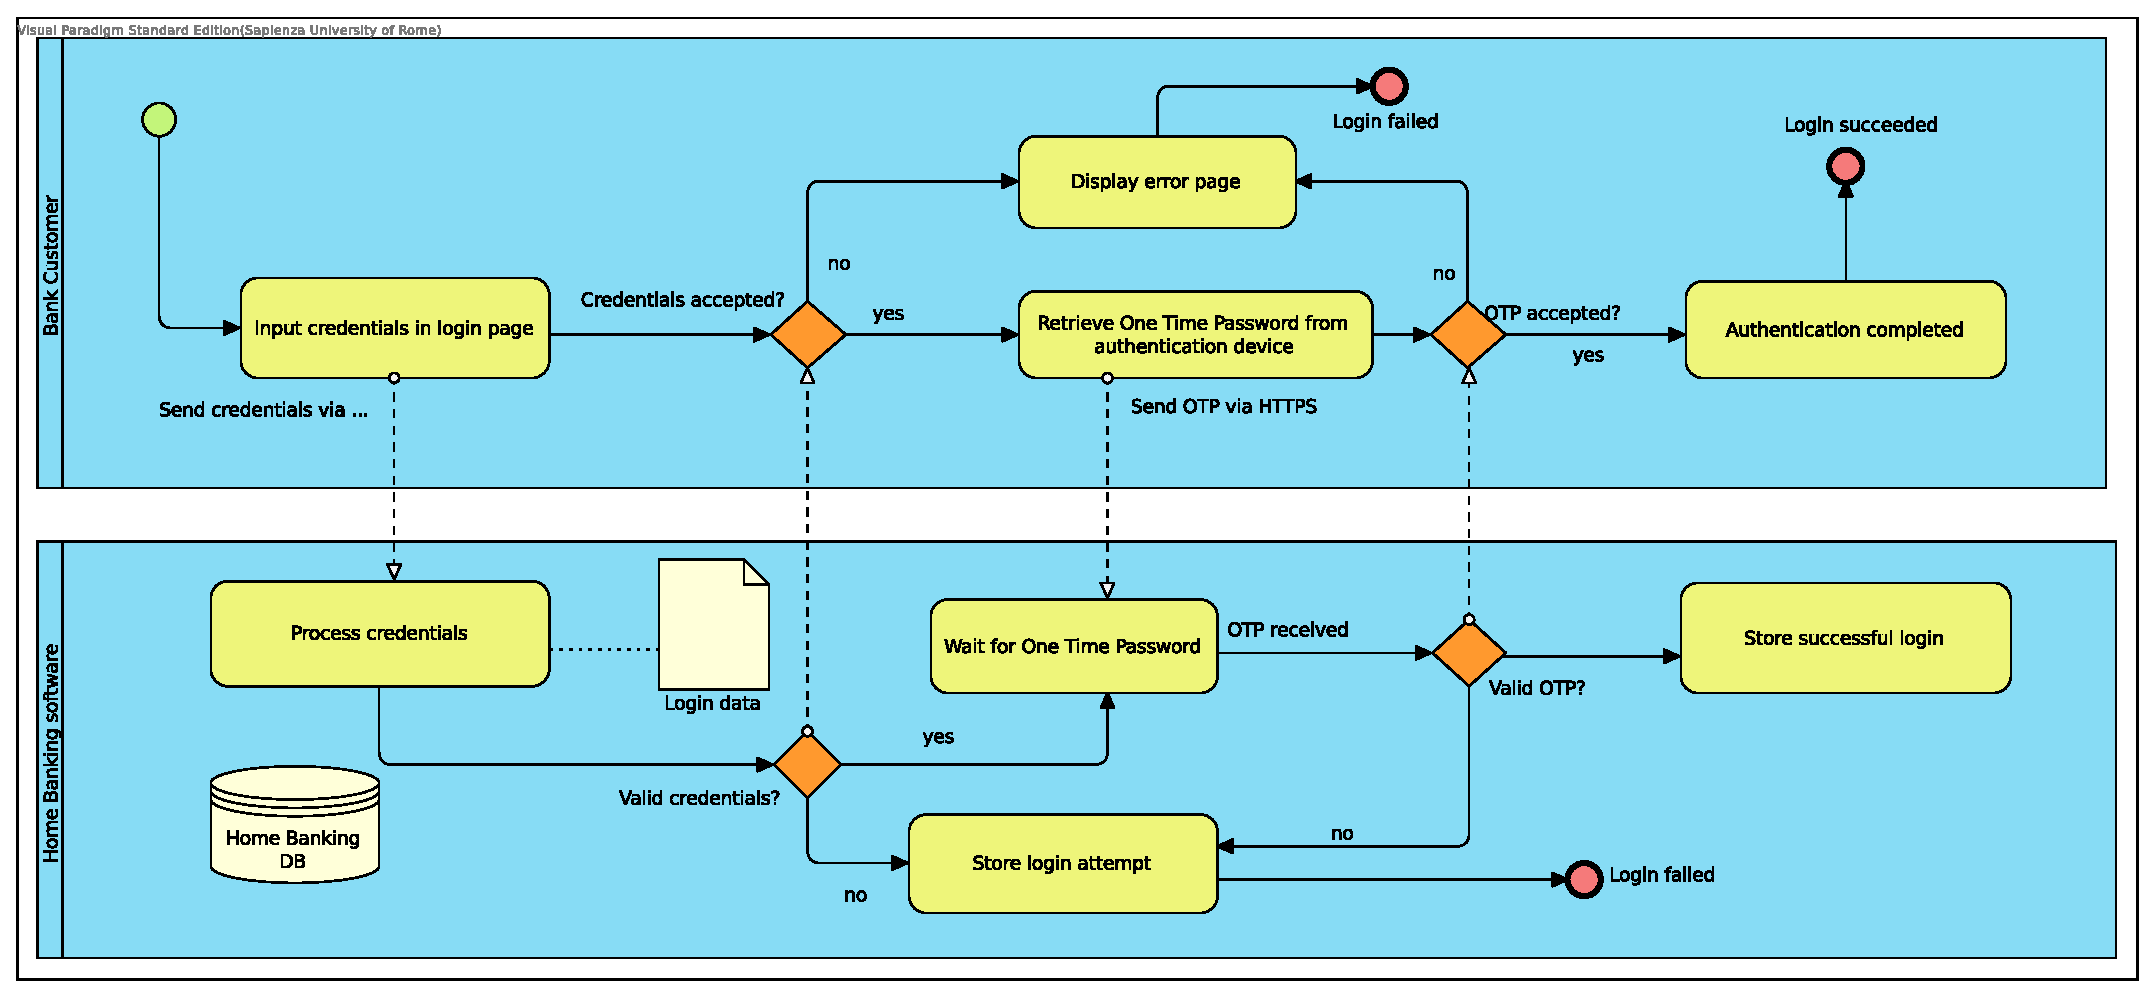
\includegraphics[width=\textheight, angle=90]{Images/Authentication.eps}
%	\caption{Business case: procedura di autenticazione.}
%	\label{fig:business_case_authentication}
%\end{figure*}
%
%\begin{figure*}[hbt]
%	\centering
%	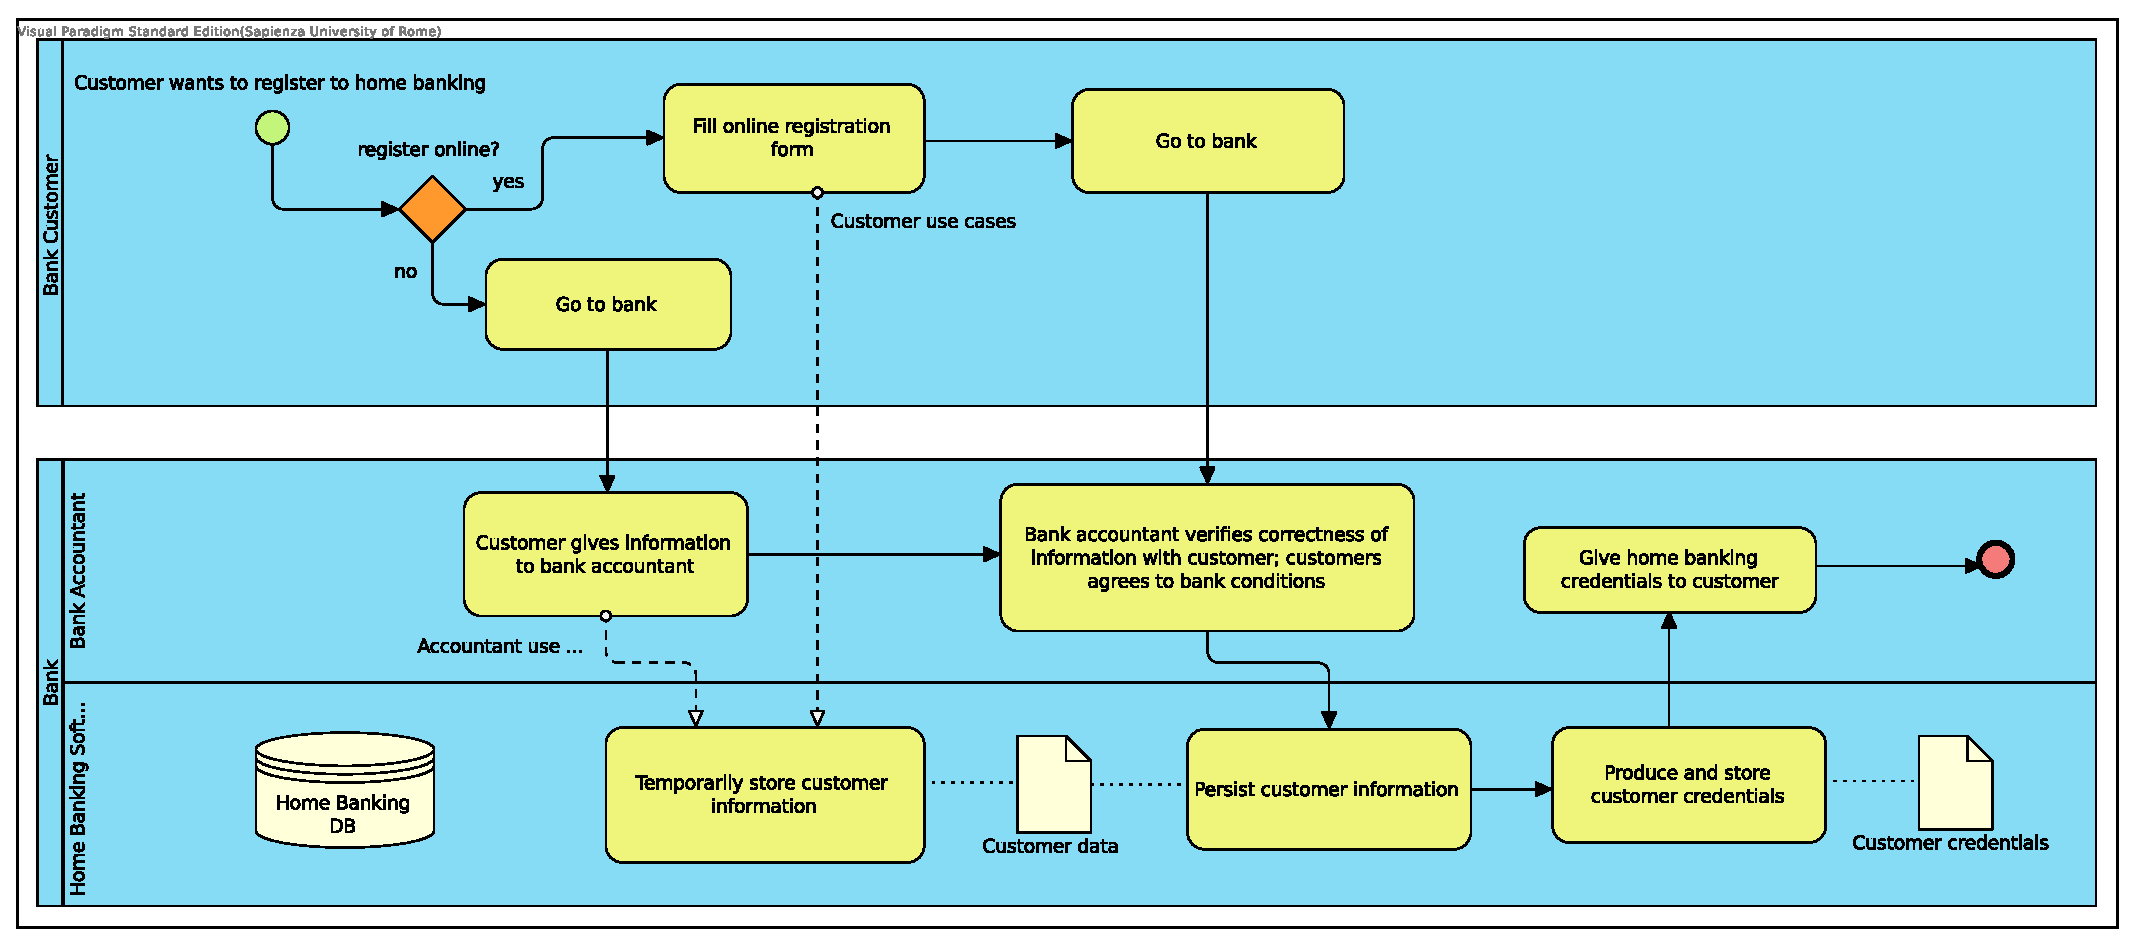
\includegraphics[width=\textheight, angle=90]{Images/Home_Banking_registration.eps}
%	\caption{Business case: procedura di autenticazione.}
%	\label{fig:business_case_authentication}
%\end{figure*}

\end{document}